\section{Algorithm Compiler}\label{sec:compiler}
\begin{figure}
  \centering
  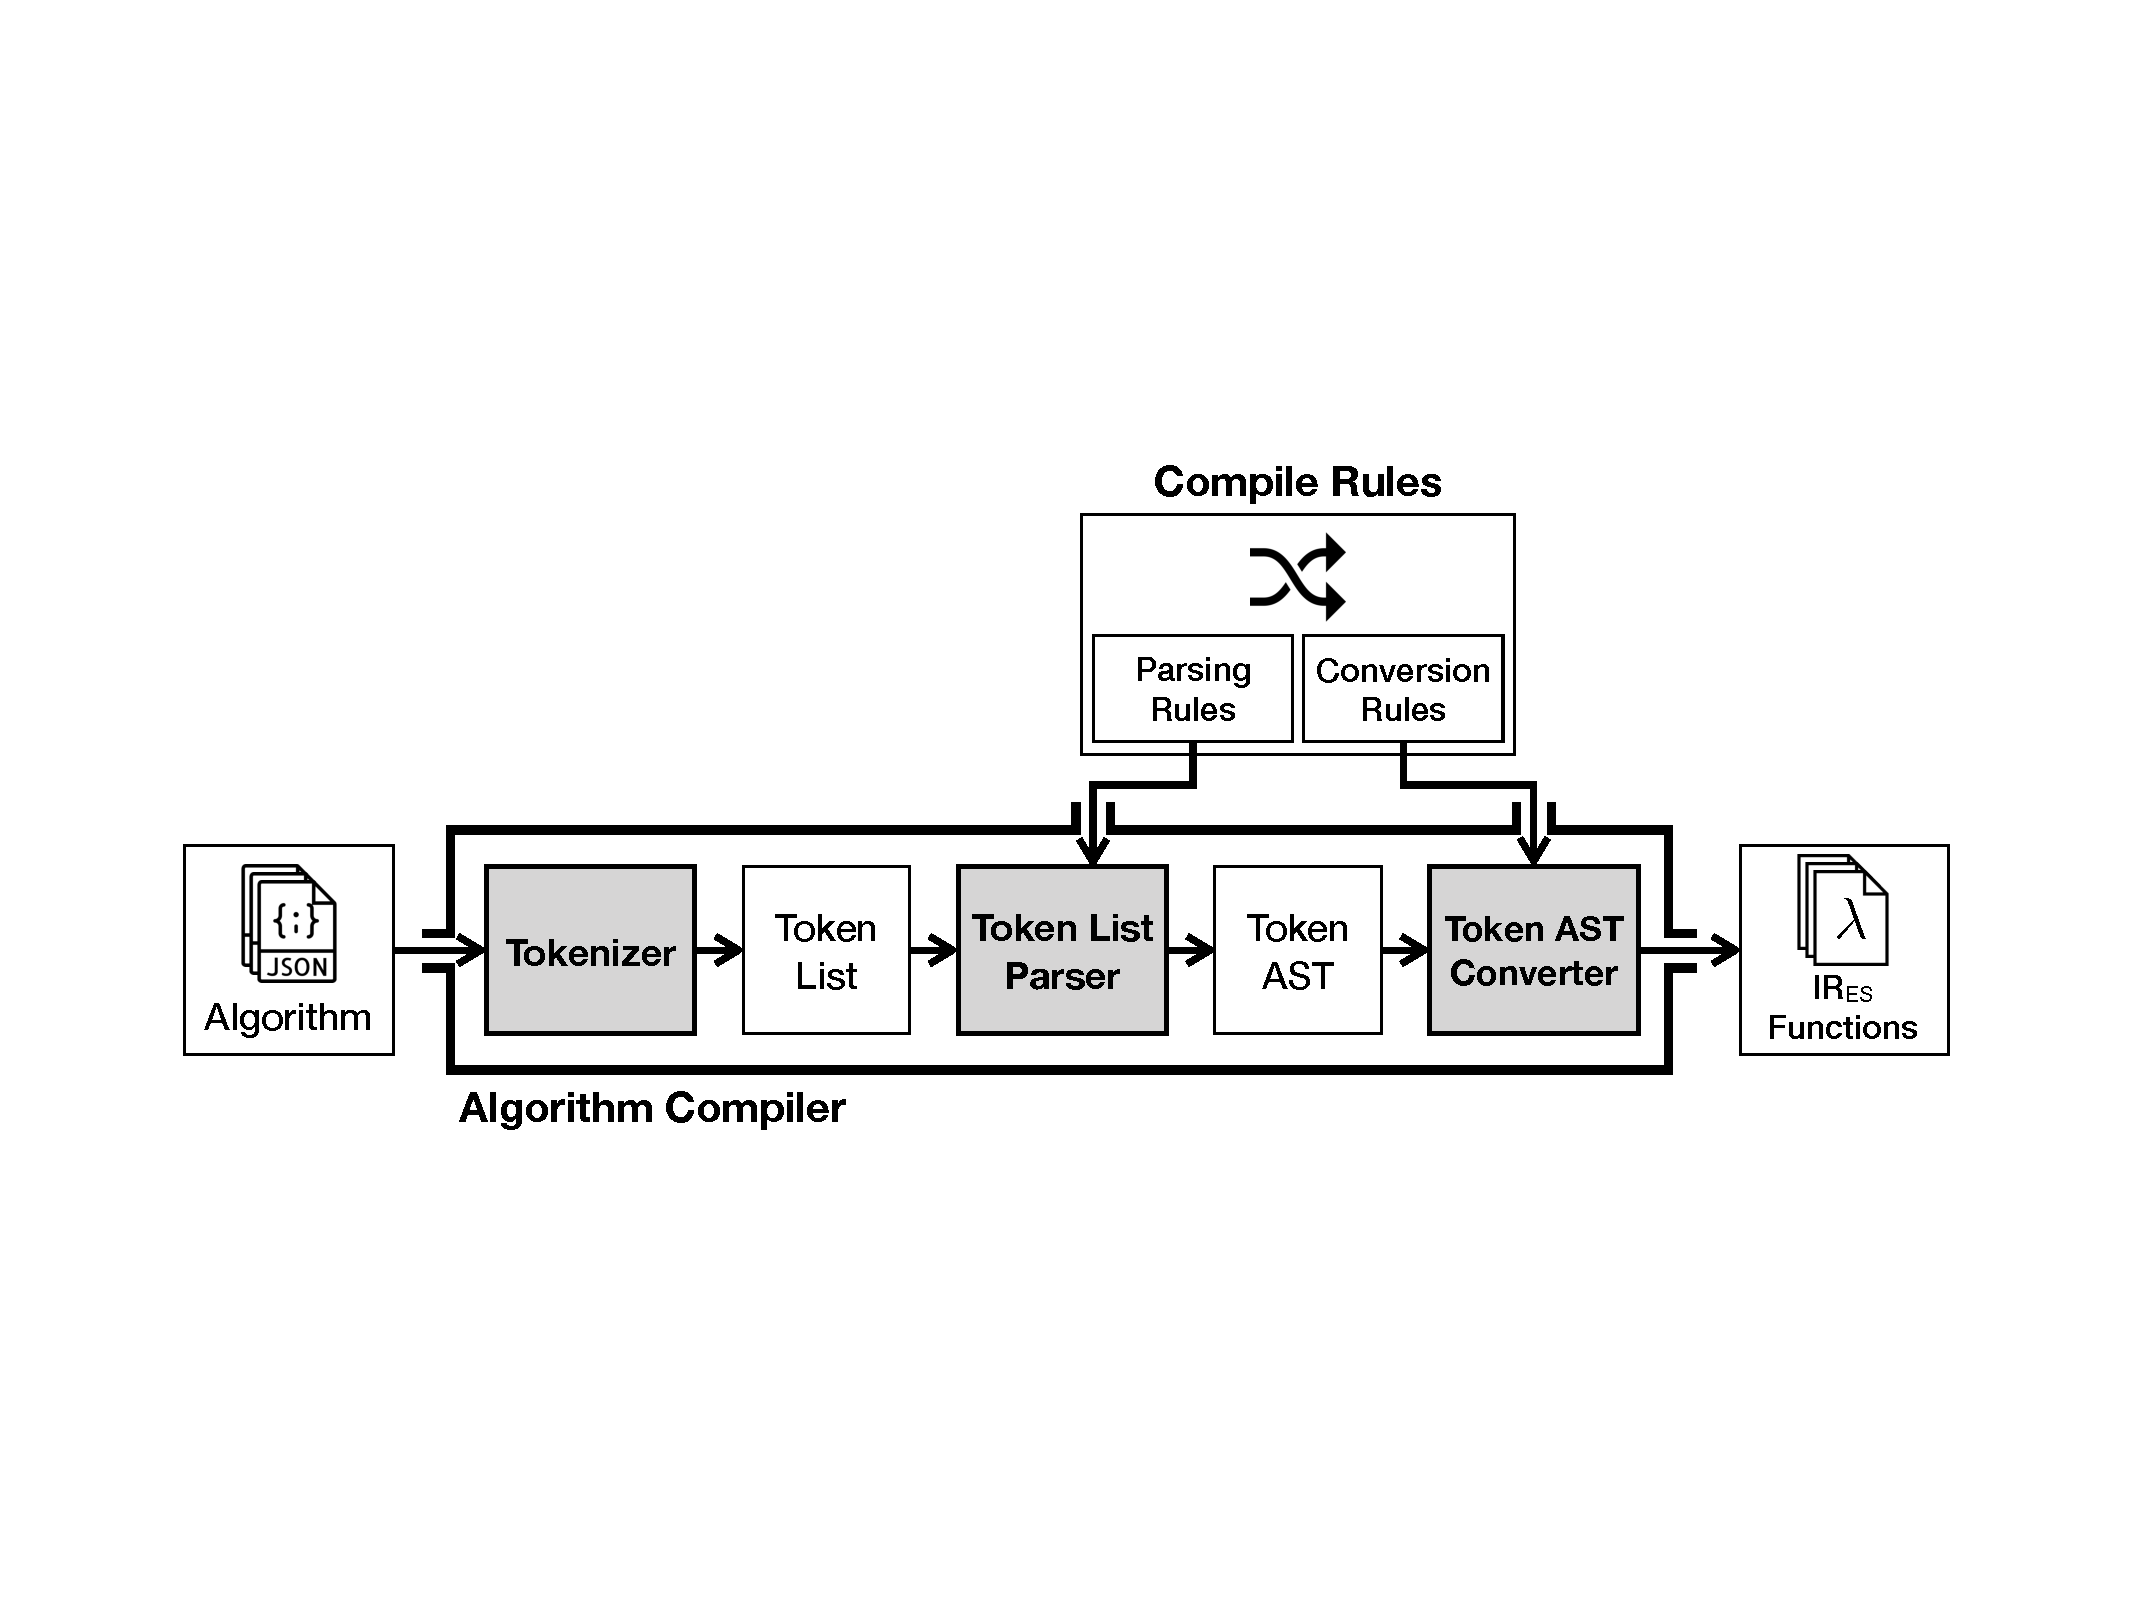
\includegraphics[width=0.48\textwidth]{img/algo-compiler.pdf}
  \caption{overall structure of {\sf algorithm compiler}}
  \label{fig:algo-compiler}
\end{figure}

In this section, we explain {\sf Algorithm Compiler} that compiles
abstract algorithms to \( \ires \) functions as illustrated in
Figure~\ref{fig:algo-compiler}.

\subsection{Tokenizer}
Before compiling abstract algorithms, {\sf Tokenizer} first tokenizes each
abstract algorithm into a list of tagged tokens.  An algorithm consists of
ordered steps, and a step may contain sub-steps as well.  For example, the
\textbf{\small Evaluation} abstract algorithm in
Figure~\ref{fig:array-literal-eval}(a) has seven steps.  Moreover, the tokens of
each step have their own HTML tags and each tag has a meaning.  We keep such
HTML tag information for each token to construct more precise {\sf Compile
Rules}. If an HTML element is just a text without any explicit tags, it is
divided into multiple tokens and each token becomes a sequence of alphanumeric
characters or a single non-alphanumeric character.  For example, in the
\textbf{\small Evaluation} algorithm, \( \textbf{\code{"length"}} \) is a single
token with the HTML tag \( \code{<code>} \) and \( \code{Perform Set(} \) is
divided into three text tokens \( \code{Perform} \), \( \code{Set} \), and \(
\code{(} \).

Moreover, {\sf Tokenizer} flattens a structured step to a single token
list to handle multi-step statements easily.  Some statements in
abstract algorithms consist of multiple steps.  For example, the
\( \code{if}\!-\!\code{then}\!-\!\code{else} \) statement often consists of
two steps: one for the \( \code{then} \)-branch and another
for the \( \code{else} \)-branch.  To treat them as a linear structure,
we introduce three special tokens to break down structured algorithms:
\( \tend \) denotes the end of a single step, and \( \tin \) and
\( \tout \) denote the start and the end of nested steps, respectively.
For example, the following left abstract algorithm is tokenized to the right
token list.
\[
  \begin{array}{lcl}
    \code{1. A}\\
    \code{2. B} &\Longrightarrow& \code{A} \tend \code{B} \tin \code{C} \tend \tout \tend\\
    \code{\ \ a. C}\\
  \end{array}
\]

After tokenizing abstract algorithms, {\sf Algorithm Compiler}
compiles token lists into \( \ires \) functions using
{\sf Token List Parser} and {\sf Token AST Converter}.
They depend on {\sf Compile Rules} and each compile rule
consists of a \textit{parsing rule} and a \textit{conversion rule}:
\begin{lstlisting}[style=myScalastyle]
val CompileRule = ParsingRule ^^ ConversionRule
\end{lstlisting}
For each compile rule, its parsing rule describes how to parse a given
token list into a structured token AST, and its conversion rule describes
how to convert the given token AST structure into an \( \ires \) component.
Now, we explain the token list parser and token AST converter with
parsing rules and conversion rules, respectively.


\subsection{Token List Parser}
The token list parser is defined with \textit{parsing rules} written in extended
Scala parser combinators. We modified the meaning of the alternative composition
operator ( \( | \) ) to collect all the longest matched results. If a parser
detects a step that cannot be parsed or parsed in multiple ways, it reports the
step with the parsing results.  We use Packrat parsing~\cite{packrat} for
parsing rules, which support left recursion.

We provide two kinds of basic parsing rules: \textit{tag-based rules} and
\textit{content-based rules}.  A tag-based rule just checks whether the next
token has a given tag.  For example, the tag-based parser \( \code{varT} \) and
\( \code{codeT} \) check whether the next token has the tag \( \code{<var>} \)
and \( \code{<code>} \), respectively.  A content-based parser checks whether
the next token is a text token and its content passes a given condition.  For
example, the string literal \( \code{"Perform"} \) denotes a content-based
parser that checks whether the next token is a text token with the content \(
\code{Perform} \).  We also provide two content-based parsers \( \code{word} \)
and \( \code{number} \) that check whether the content of the next token
consists of only alphabets or numbers, respectively.  In parsing rules, all the
helper functions defined in Scala parser combinators are available.  For
instance, the helper function \( \code{repsep(p, q)} \) generates a new parsing
rule that denotes zero or more repetition of the parsing rule \( \code{p} \)
using another parsing rule \( \code{q} \) as a separator.

Consider the following example parsing rule for the step 5 of the
\textbf{Evaluation} algorithm in Figure~\ref{fig:array-literal-eval}(a).
\begin{lstlisting}[style=myScalastyle]
// statements
val Stmt = "Perform" ~ Expr ~ "." ^^ ...
// expressions
val Expr =
  // codes        // false literal
  codeT    ^^ ... |  "false"           ^^ ... |
  // variables       // additions
  varT     ^^ ... |  Expr ~ "+" ~ Expr ^^ ... |
  // function calls
  word ~ "(" ~ repsep(Expr, ",") ~ ")" ^^ ...
\end{lstlisting}
We omit the conversion rule for each compile rule for the brevity.  The \(
\code{Stmt} \) compile rule  describes how to compile statements with a single
parsing rule, and the \( \code{Expr} \) compile rule describes how to compile
expressions with five parsing rules.  A token parser with the above rules parses
the step 5 of \textbf{Evaluation} to the following token AST:
\begin{center}
  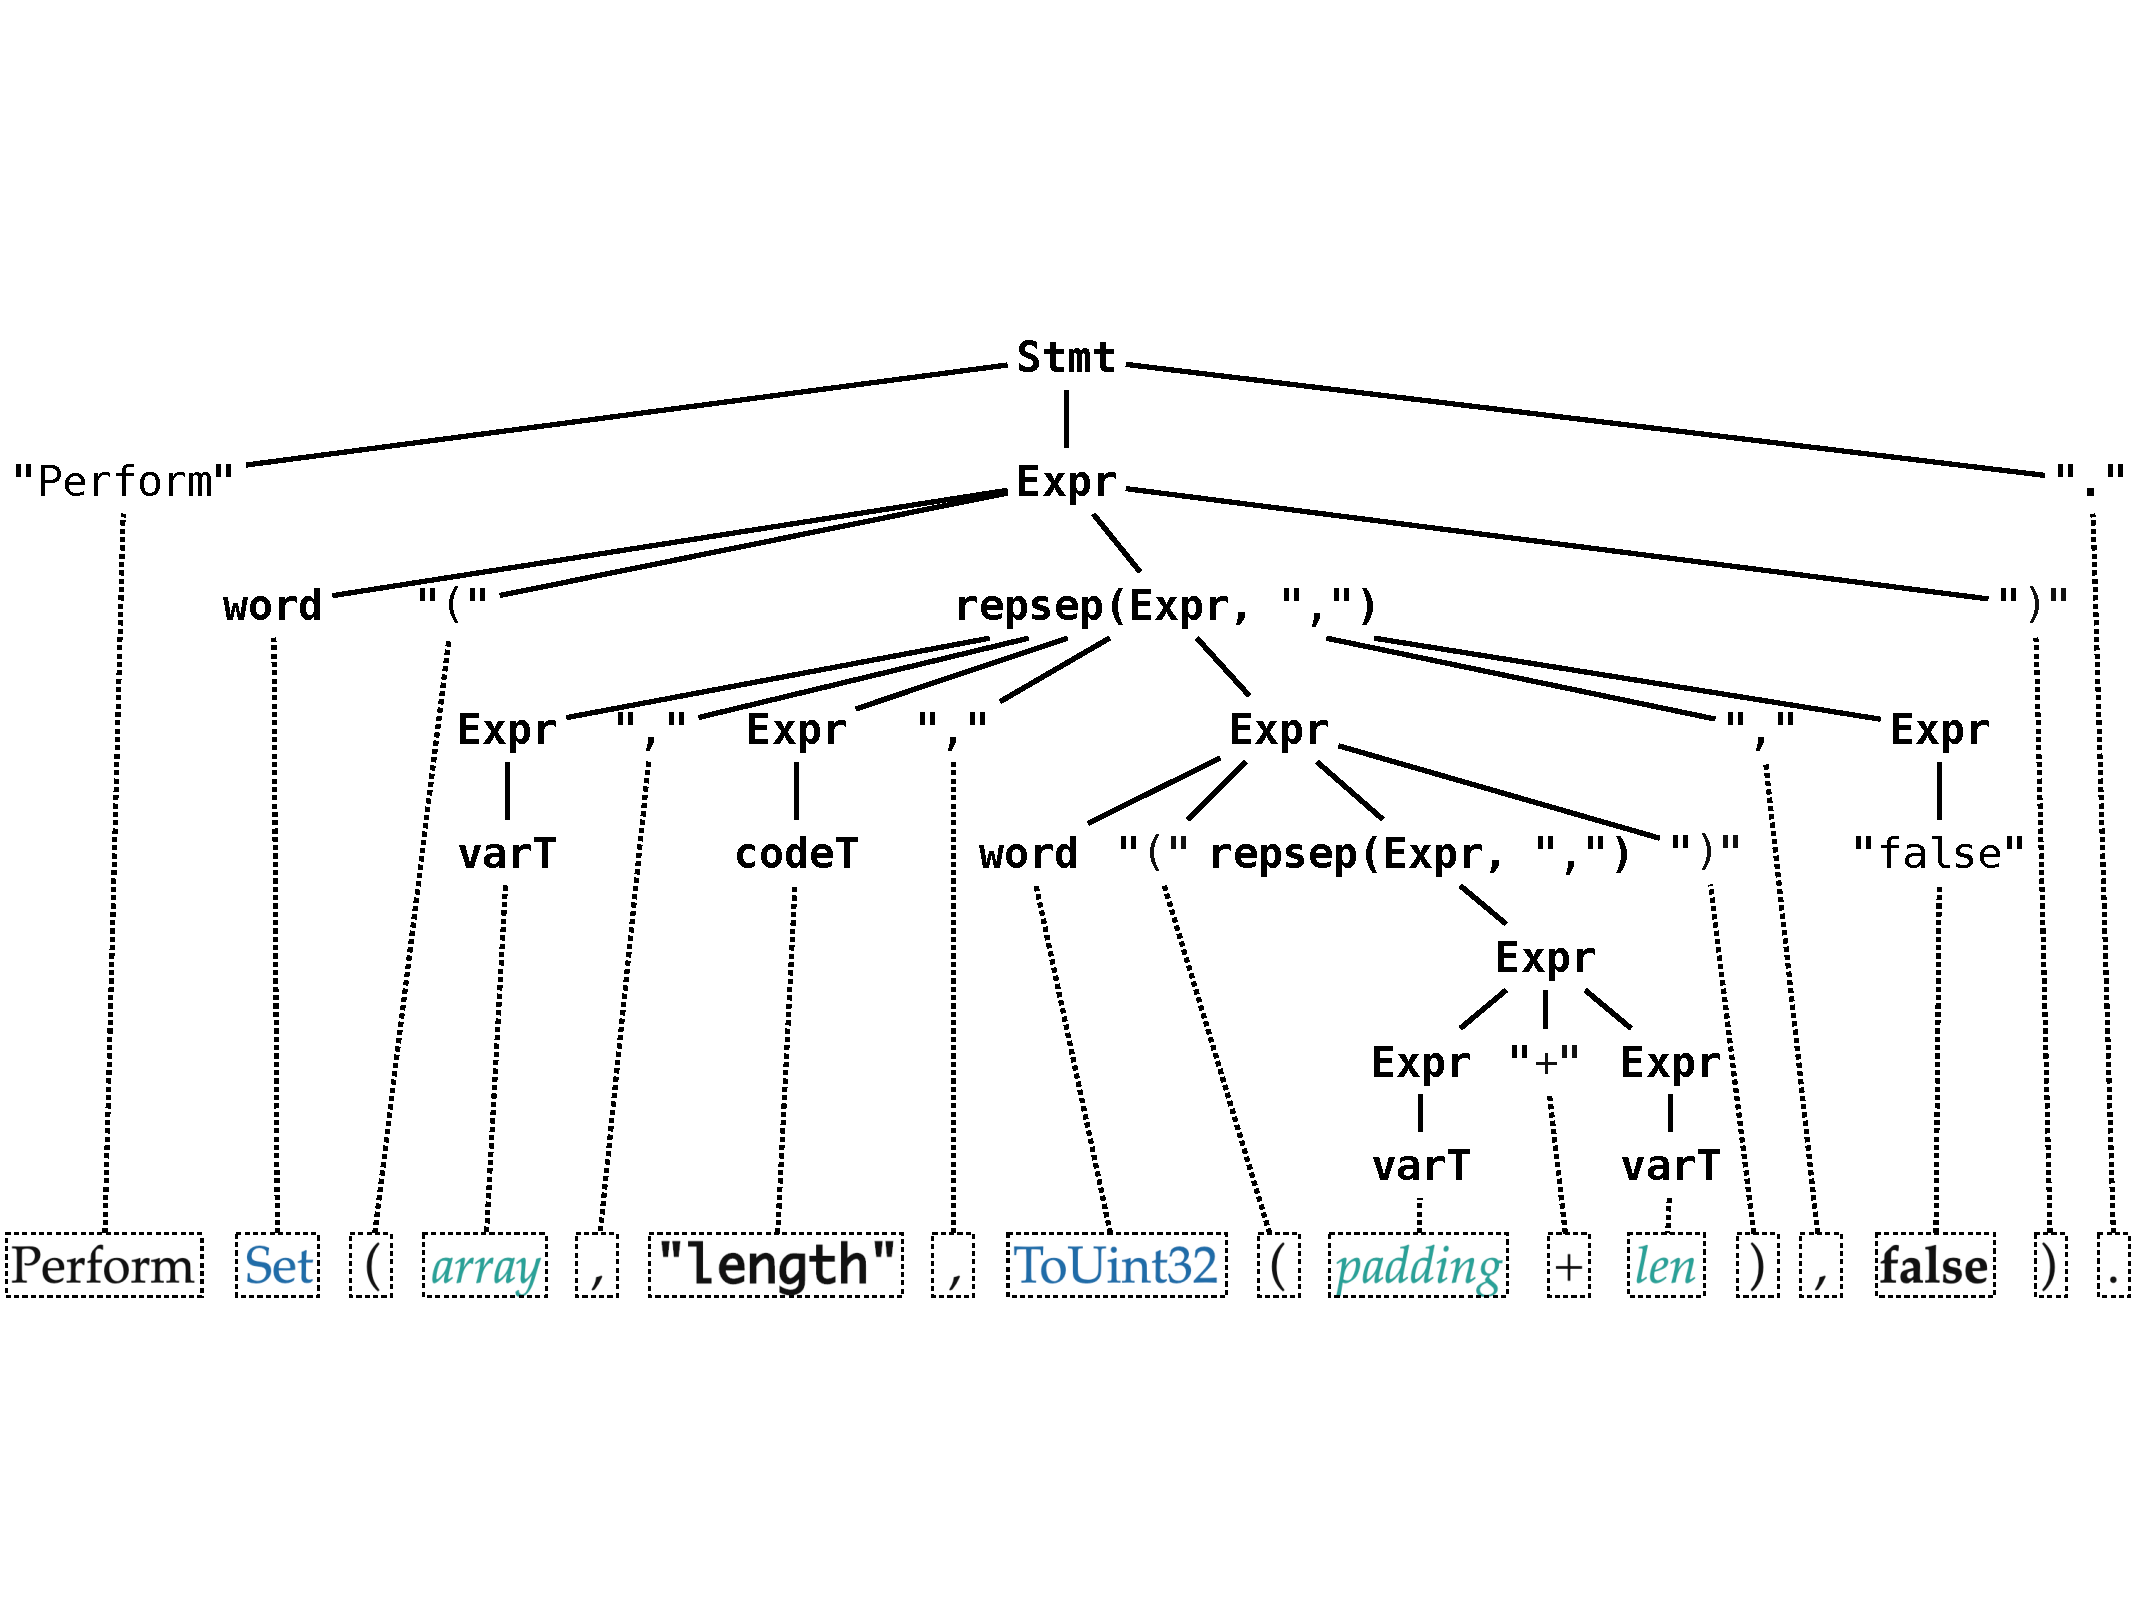
\includegraphics[width=0.5\textwidth]{img/token-ast.pdf}
\end{center}


\subsection{Token AST Converter}
\textit{Conversion rules} describe how to generate an \( \ires \) function for a
given token AST.  Each conversion rule is defined with its corresponding parsing
rule.  For basic parsing rules, their conversion rules always return the string
values of the contents in parsed tokens.  For example, the following conversion
rules are the omitted parts in the previous example for the step 5 of
\textbf{Evaluation}:
\begin{lstlisting}[style=myScalastyle]
// statements
val Stmt = ... ^^ { case _ ~ e ~ _ => IExpr(e) }
// expressions
val Expr =
  // codes      // false literal
  ... ^^ EStr | ... ^^ { _ => EBool(false) } |
  // variables  // additions
  ... ^^ EId  | ... ^^ { case x ~ _ ~ y => EAdd(x, y) } |
  // function calls
  ... ^^ { case x ~ _ ~ y ~ _ => ECall(x, y) }
)
\end{lstlisting}
The conversion rule of the \code{Stmt} compile rule uses only the second sub
tree and constructs an \code{IExpr} \( \ires \) instruction.  For the second
sub-tree, the conversion rule of the fourth \code{Expr} compile rule is
applied. It constructs \code{ECall} \( \ires \) expression with the string value
of the first sub-tree and the sequence of the expressions of the third sub-tree.
In this way, the step 5 of \textbf{Evaluation} is converted to the following \(
\ires \) instruction:
\begin{lstlisting}[style=ires]
(Set array "length" (ToUint32 (+ padding len)) false)
\end{lstlisting}

We define \( \ires \) to represent abstract algorithms as its
functions with the following design choices:
\begin{itemize}[leftmargin=0.5cm]
\item \textbf{Dynamic typing:} Because each variable in abstract
algorithms is not statically typed, variables do not have their own
static types while each value of \( \ires \) has its dynamic type.

\item \textbf{Imperative style:} \( \ires \) represents algorithm steps
as imperative instructions in the sense that each instruction changes
the current state consisting of an environment and a heap.

\item \textbf{Higher-order functions with restricted scopes:}
In each function of \( \ires \), only global variables, parameters,
and its local variables are available, which means that a function
closure does not capture its current environment.  We use such
restricted scopes because they are enough to represent abstract
algorithms.

\item \textbf{Primitive values:} \( \ires \) supports ECMAScript primitive
values except ``symbols'' because symbols can be represented as singleton
objects.  Also, \( \ires \) provides the unique \( \code{absent} \) value to
represent the absence of parameters.  For example, when the optional second
parameter \textit{Elision} of \textbf{Evaluation} in
Figure~\ref{fig:array-literal-eval}(a) is absent, the parameter has the \(
\code{absent} \) value.

\item \textbf{Abstract data types:} \( \ires \) supports only three abstract
data types: \( \code{Record} \) for mappings from some values to other values,
\( \code{List} \) for sequential data, and \( \code{Symbol} \) for singleton
data.  For example, ECMAScript environment records are represented as \(
\code{Record} \) from string values into addresses that represent other types
of \( \code{Record} \) for bindings.
\end{itemize}
We define syntax of \( \ires \) consisting 15 kinds of instructions and 26 kinds
of expressions with the notation \( \irinst \) and \( \irexpr \), respectively.
Moreover, we also formally define their operational semantics with the form \(
\irstate \vdash \irinst \Rightarrow \irstate \) for instructions, and the form
\( \irstate \vdash \irexpr \Rightarrow (\irvalue, \irstate) \) for expressions
where \( \irvalue \) denotes a value and \( \irstate \) denotes a state.
However, we omit this formalization in this paper for brevity, instead, we
include it in the companion material\footnote{\inred{???}}.
